\chapter{Supersimetría}

\hll{Agregar introduccion}

\section{Motivación}

El {\SM} de la física de altas energías descripto en el capítulo anterior,
con el agregado de la masa de los neutrinos, y el descubrimiento del bosón
de Higgs, ha tenido un gran éxito en la descripción de los fenómenos
conocidos hasta la escala del {\tev} a la que los experimentos han llegado
en los últimos a\~nos.
%% A pesar de esto, resulta claro que el Modelo Est\'andar no es una teoria definitiva y va a tener que
%% ser extendida para describir la f\'isica de altas energ\'ias.
A pesar de esto, no hay dudas respecto a que una nueva teor\'ia va a ser
necesaria a la escala reducida de Planck %% $M_P =  (8\pi G_\text{Newton})^{-1/2} = 2.4 \times 10^{18} \gev$ ,
donde los efectos cu\'anticos gravitacionales son importantes. Sabemos que
que tiene que existir nueva f\'isica en los 16 ordenes de magnitud en
energ\'ia entre el territorio explorado cerca de la escala electrod\'ebil
y la escala de Planck.
El s\'olo hecho de que la relación $M_P/M_W$ es tan grande es una gran pista
para la física mas allá del {\SM}, por el llamado \emph{problema de jerarquía}.
Este no es una dificultad intrínseca del {\SM}, sino una sensibilidad \hl{diusturbing}
del potencial de Higgs a nueva fisica en casi cualquier extension imaginable
del SM.
La parte eléctricamente neutra del campo de Higgs del SM es un escalar complejo
$H$ con un potencial clásico $V=m_H^2 |H|^2 + \lambda|H|^4$.
El SM necesita un valor de expectación del vacío (VEV) para $H$ en el
mínimo del potencial no nulo.
Esto ocurre si $\lambda>0$ y $m_H^2<0$, resultando en
$\avg{H} = \sqrt{-m_H^2/2\lambda}$.
Como experimentalmente sabemos que $\avg{H}$ es aproximadamente 174 \gev,
de las medidas de las propiedades de las interacciones débiles, el valor de
$m_H^2$ debe ser del orden de $-(100 \gev)^2$.

\begin{figure}[h]
  \centering
  \begin{tikzpicture}[node distance=1cm and 1 cm]

  \coordinate[vertex, label=above:$H$] (v1);
  \coordinate[vertex, right=of v1] (v2);
  \coordinate[vertex, right=of v2] (v3);
  \coordinate[vertex, right=of v3] (v4);

  \draw[higgs] (v1) -- (v2);
  \draw[higgs] (v3) -- (v4);

  \draw[fermion] (1.5, 0) circle (0.5);
  \node at (1.5, 0.75) {$f$};

\end{tikzpicture}

  \caption{Correciones cu\'anticas a un loop al cuadrado de la masa del Higgs
    $m_H^2$ debido a la masa de un fermi\'on de Dirac $f$.}
  \label{fig:higgs_correction_f}
\end{figure}

El problema es que $m_H^2$ recibe grandes correcciones cuánticas de los efectos
virtuales de cada partícula a la cual se acopla, directa o indirectamente, al
campo de Higgs. Por ejemplo, en la \cref{fig:higgs_correction_f} tenemos una
corrección a $m_H^2$ del loop que contiene un fermión de Dirac $f$ con masa
$m_f$. Si el campo de Higgs se acopla a $f$ con un término en el lagrangiano
igual a $-\lambda_f H \bar{f}f$, el diagrama de Feynman en la
\cref{fig:higgs_correction_f} genera una corrección:

\begin{equation}
  \Delta m_H^2 = -\frac{|\lambda_f|^2}{8\pi^2} \Lambda^2_\text{UV} + \ldots
  \label{eq:higgs_corr_f}
\end{equation}
%
donde $\Lambda_\text{UV}$ es el corte usado para regular la integral en el
\emph{loop}.
Debe ser interpretado como la m\'inima escala de energ\'ia a la cual entra
la nueva física para alterar el comportantamiento de la teoría a altas
energías. Los puntos suspensivos representan terminos proporcionales a
$m_f^2$, que crecen a lo sumo logaritmicamente con $\Lambda_\text{UV}$.
Cualquiera de los leptones o quarks del SM puede jugar el rol de $f$ (para
el caso de quarks la correcci\'on tiene que ser multiplicada por 3 para
tener en cuenta el color) y la correci\'on m\'as grande va a ser cuando
$f$ es el quark \emph{top} con $\lambda_f \approx 1$.

El problema aparece si $\Lambda_\text{UV}$ es del orden de $M_P$, ya que
la correci\'on a $m_H^2$ es 30 ordenes de magnitud mas grande que el valor
requerido de $m_H^2 \sim (100 \gev)^2$.
Este es sólo un problema para las correcciones al cuadrado de la masa del
bos\'on de Higgs escalar, porque las correcciones cuanticas a las masas de
los fermiones y los bosones de gauge no tienen una sensibilidad cuadratica
directa a $\Lambda_\text{UV}$ como la que estan en la \cref{eq:higgs_corr_f}.
Sin embargo, los quarks, leptones y los bosones de gauge electrodebiles
$Z^0$, $W^{\pm}$ del SM, todos obtienen masa de $\avg{H}$, por lo tanto el
espectro completo de masas del SM es directa o indirectamnte sensible a
la escala de corte $\Lambda_\text{UV}$.

Uno puede pensar que la soluci\'on es elegir un $\Lambda$ no demasiado
grande. Pero igual uno todavia deberia mezclar algo de neuva fisica
a la escala $\Lambda_\text{UV}$ que no solo altere los propagadores en
el loop, sino que corte la integral. Esto no es facil en una teoria cuyo
lagrangiano no conitene mas de dos derivadas, y las teorias de mayor orden
en derivadas generalmente sufren de fallas de unitariedad o causalidad.
%In string theories, loop integrals are nevertheless cut off at high Euclidean
%% momentum p by factors e −p /Λ UV . However, then Λ UV is a string scale that is usually † thought to be
%% not very far below M P . Furthermore, there are contributions similar to eq. (1.2) from the virtual effects
%% of any arbitrarily heavy particles that might exist, and these involve the masses of the heavy particles,
%% not just the cutoff.

\begin{figure}[h]
  \centering
  \begin{tikzpicture}[node distance=1cm and 1 cm]

  \coordinate[vertex, label=above:$H$] (v1);
  \coordinate[vertex, right=of v1] (v2);
  \coordinate[vertex, right=of v2] (v3);
  \coordinate[vertex, right=of v3] (v4);

  \draw[higgs] (v1) -- (v2);
  \draw[higgs] (v2) -- (v3);
  \draw[higgs] (v3) -- (v4);

  \draw[higgs] (1.5, 0.5) circle (0.5);

  \node at (1.5, 1.25) {$S$};

\end{tikzpicture}

  \caption{Correciones cu\'anticas a un loop al cuadrado de la masa del
    Higgs $m_H^2$ debido a la masa de un campo escalar $S$.}
  \label{fig:higgs_correction_s}
\end{figure}

En el caso de que exista un escalar complejo pesado $S$ con masa $m_S$
que se acopla al Higgs con un termino en el Lagrangiano
$-\lambda_S \abs{H}^2 \abs{S}^2$, el diagrama de Feynman es el que se
muestra en la \cref{fig:higgs_correction_s} y este da lugar a una
corrección:

\begin{equation}
  \Delta m_H^2 = \frac{\lambda_S^2}{16\pi^2} \left[ \Lambda^2_\text{UV} - 2 m_S^2 \ln (\Lambda^2_\text{UV}/m_S) +  \ldots \right]
  \label{eq:higgs_corr_s}
\end{equation}

%% Puede ser que el boson de Higgs no sea una fundamenta, como en modelos technicolor, o modelos en
%% los cuales el Higgs es compuesto.
Si el bosón de Higgs es una partícula fundamental y hay física a una
escala mucho mayor a la escala electrodébil, existen dos opciones:
tenemos que hacer alguna asumpcion bizarra que no existe ninguna
partícula de mayor masa o efectos que se acoplen (incluso indirectamente
o extremadamente débiles) con el campo escalar de Higgs, o algún tipo
de  cancelación es necesaria entre las varias contribuciones a $\Delta m_H^2$.

%------
% SUSY
%------
\section{Supersimetría}

La cancelación sistemática de las contribuciones a $\Delta m_H^2$ puede
ser realizada por una simetría. Comparando las \cref{eq:higgs_corr_f,eq:higgs_corr_s}
se puede ver que la nueva simetría tiene que relacionar bosones y fermiones,
debido al signo menos entre las contribuciones del loop fermionico y el
bosonico.

Afortunadamente la cancelación de todas estas contribuciones a las masas
escalares no solo es posible, sino que es inevitable, si consideramos
que existe una simetría que relaciona fermiones y bosones.
A esta simetría la llamamos supersimetría o SUSY.

Una transformación supersimétrica convierte un estado bosónico en uno
fermiónico, y viceversa. El operador $Q$ que genera estas transformaciones
debe ser un spinor anticonmutativo, con

\begin{equation}
  Q \ket{\text{bosón}} = \ket{\text{fermión}}, \quad \quad Q \ket{\text{fermión}} = \ket{\text{bosón}}
\end{equation}

Los espinores son intrínsecamente objectos complejos, por lo tanto el conjugado
hermitico de $Q$ es también un generador de la simetría. Debido a que $Q$ y $Q^\dagger$
son operadores fermiónicos, llevan momento angular de spin 1/2, por lo tanto es
claro que SUSY debe ser una simetria espacio-temporal y los operadores $Q$ y
$Q^\dagger$ deben satisfacer un algebra de la siguiente forma,

\begin{align}
  \{Q, Q^\dagger\} &= P^\mu \\
  \{Q, Q\} &= \{Q^\dagger, Q^\dagger\} = 0 \\
  [P^\mu, Q] &= [P^\mu, Q^\dagger] = 0 \\
\end{align}
%
donde $P^\mu$ es el cuadrimomento generador de las traslaciones espacio-temporales.

Los estados de partícula de una teoría supersimétrica son representados en
el álgebra de SUSY como \emph{supermultipletes}. Cada supermultiplete contiene
ambos estados, fermión y bosón, que son comúnmente llamados supercoma\~neros
uno de otro.

Los generadores $Q$ y $Q^\dagger$ conmutan con los generadores de las
transformaciones de gauge, por lo tanto las partículas en un mismo supermultiplete
tienen que estar en la misma representación del grupo de gauge, y tener la misma
carga eléctrica, isospin y color. El operador de masa $-P^2$ también conmuta con los
generadores y con todos los operadores de rotación y traslación, por lo tanto las
partículas que habiten el mismo supermultiplete deben tener los mismos autovalores
de $-P^2$, y entonces la misma masa.

Es fácil probar que cada supermultiplete tiene que contener igual numero de grados
de libertad fermiónico que bosónico, $n_B = n_F$.
La posibilidad mas simple para satisfacer esto es tener un único fermión de Weyl
($n_F=2$) y dos escalares reales (cada uno con $n_B=1$). Es natural poner estos
dos escalares en un único campo escalar complejo. Esta combinación de un fermión
de Weyl de dos componentes y un campo escalar complejo es llamado un supermultiplete
\emph{quiral} (o \emph{escalar} o de \emph{materia}).


Otra posibilidad es
que el supermultiplete contenga un bosón vectorial de spin 1. Para que la teoría
sea renormalizable, tiene que ser un bosón de gauge no masivo, al menos antes de
que la simetría de gauge sea espontáneamente rota. En este caso, este bosón contiene
dos estados de helicidad, $n_B=2$. Por lo tanto su supercomanero es un fermión de Weyl
de spin 1/2, con dos estados de helicidad, $n_F=2$. Si en vez de esto, uno intenta usar
un fermión de spin 3/2 la teoría no seria renormalizable. Los bosones de gauge deben
transformar como la represnetacion adjunta del grupo de gauge, por lo que sus compañeros
fermiónico, llamados \emph{gauginos}, también. Estas combinaciones de gauginos de
spin 1/2 y bosones de gauge de spin 1 es llamada supermultiplete de \emph{gauge} o
\emph{vectorial}.

Si incluimos la gravedad, el graviton de spin 2 (con dos estados de helicidad, $n_B=2$)
tiene un supercomanero de spin 3/2 llamado \emph{gravitino}.

Existen otras combinaciones posibles de particulaes que pueden satisfacer esta
condicion, pero siempre se reducen a combinaciones de supermultipletes quirales
de o de gauge, excepto en ciertas teorias con supersimetria extendida. Estas
teorias tuenbe mas de una copia de los generadores $Q, Q^\dagger$, pero no son
muy prometedoras desde el punto de vista fenomenologigo.
La teoria no extendida y fenologicamente viable es llamada generalmente $N=1$,
donde $N$ se refiere al numero de supersimetrias (el numero de las distintas
copias de $Q,Q^\dagger$).


%------
% MSSM
%------
\section{Modelo Mínimo Estándar Supersimétrico}

En una extensión supersimétrica del SM, cada una de las partículas fundamentales
conocidas esta contenida en un supermultiplete quiral o de gauge, y debe tener
un supercoma\~nero con spin que difiere en 1/2.
La extensión que requiere la introducci\'on de la minima cantidad de
partículas es llamado \emph{Modelo Mínimo Estándar Supersimétrico}, o MSSM.

%% The first step in understanding the exciting phenomenological consequences of
%% this prediction is to decide exactly how the known particles fit into supermultiplets, and to give them
%% appropriate names.

Solo los supermultipletes quirales pueden contener fermiones cuya parte izquierda
y derecha transforman de forma diferente bajo el grupo de gauge.
Todos los fermiones del SM (quarks y leptones) tienen esta propiedad,
por lo tanto deben ser miembros de supermultipletes quirales.
Los nombres de los companeros de spin 0 de los quarks o leptones son construidos
anteponiendo una ``s'' (de \emhp{scalar}). Por lo tanto son llamados \emph{squarks}
y \emph{sleptones}, o \emph{sfermiones}. Y se utiliza el mismo simbolo con un tilde.
La parte izquierda y derecha de los quarks y leptones son fermiones de Weyl
con diferentes propiedades de trnasformacion de gauge del SM, entonces cada
uno debe tener un companero escalar complejo.
Por ejemplo, los supercomaneros de la parte izquierda y derecha del campo
de Direac de los electrones son llamadas parte izquierda y derecha de los
slectrones, {\selL} y {\selR}, aunque el subindice no se refiere a la
helicidad de los slectrones (tiene spin 0) sino a la de sus supercomaneros.
Lo mismo ocurre para {\smuL}, {\smuR}, {\stauL} y {\stauR}. Los neutrinos
del SM son siempre izquierdos por lo que sus supercomanero se denotan:
{\snu}. Y para los quarks tenemos {\squarkL} y {\squarkR}, con $q = u, d, s, c, b, t$.
Las interacciones de gauge de cada uno de los campos de squarks y sleptones
son las mismas que la de los correspondientes fermiones del SM.

El boson escalar de Higgs debe estar en un supermultiplete quiral ya que tiene spin 0.
Dada la naturaleza de los campos quirales introducidos en la implementación de SUSY, el campo
escalar de Higgs no es suficiente para dar masa a los fermiones de helicidad izquierda y derecha.
Se debe agregar un nuevo campo escalar para compensar. En el SM, el campo de Higgs es un doblete,
y de los cuatro grados de libertad solo uno permanece como consecuencia del rompimiento de la
simetría EW, resultando en un bos\'on de Higgs. Los dos dobletes de Higgs del MSSM son:
%
\begin{equation}
  H_u = \binom{H_u^+}{H_u^0}, \quad \quad \quad H_d = \binom{H_d^0}{H_d^-}
\end{equation}


Los bosones vectoriales del SM tienen que estar en supermultipletes de gauge.
Sus supercomaneros fermionicos son llamados \emph{gauginos}. Las interacciones
de gauge de color $SU(3)_C$ de QCD son mediadas por el gluon, cuyo companero
supersimetrico de spin 1/2 es el \emph{gluino}. La simetria electrodebil
$SU(2)_L \times U(1)_Y$ esta asociada con los bosones de spin 1 $W^+, W^0, W^-$
y $B^0$, cuyos companeros de spin 1/2 son $\susy{W}^+, \susy{W}^0, \susy{W}^-$
y $\susy{B}^0$, y llamdos \emph{winos} y \emph{bino}.
Despues de la ruptura de la simetria electrodebil, los autoestados $W^0$ y $B^0$
se mezclan para dar $Z^0$ y $\gamma$. La correspondiente mezcla de {\winozero}
y {\bino} son llamdos \emph{zino} (\zino) y \emph{fotino} (\photino).

La tabla....


\begin{figure}[h]
  \centering
  \includegraphics[width=0.9\textwidth]{figures/tabla}
\end{figure}



\subsection{El espectro de masas del MSSM}

Una característica importante del MSSM es que las súper-compañeras listadas en la
tabla no son necesariamente autoestados de masa de la teoría. Esto es porque después
del rompimiento de la simetría electrodébil y de SUSY, puede haber mezcla entre
los gauginos y higgsinos, y entre los squarks y sleptones y los Higgs escalares
que tienen la misma carga eléctrica. La única excepción es el gluino.

En el MSSM, la descripción del rompimiento de la simetría electrodéebil es un
poco mas complicada debido al hecho de que hay dos dobletes complejos de Higgs
$H_u$ y $H_d$ en vez de solo uno como en el SM.

\note{explicar minimamente el rompimiento}

%% En el MSSM los higgsinos neutros y los gauginos se mezclan para formar los cuatro neutralinos:
%% \ninoone, \ninotwo, \ninothree\ y \ninofour.
%% Y de forma similar los higgsinos cargados y los winos dan lugar a los dos charginos, \chinoonepm\ y \chinotwopm.


%% con un total de 8 grados de libertad, 3 de los cuales se pierden en el rompimiento
%% de la simetria EW. Por lo tanto quedan 5 bosones de Higgs en el MSSM: $h^0, H^0, H^+, H^-, A^0$.
%% El más liviano de los 5 es $h^0$, el cual es el más similar al del SM.


%%\subsection{Neutralinos y Charginos}

Los higgsinos y los gauginos electrodebiles se mezclan entre ellos debido al
efecto del rompimiento de la simetría electrodébil. Los higgsinos neutros
($\susy{H}_u^0$ y $\susy{H}_d^0$) y los gauginos neutros (\bino, \winozero)
se combinan para formar cuatro autoestados de masa llamados neutralinos.
Los higgsinos cargados ($\susy{H}_u^+$ y $\susy{H}_d^-$) y los winos
(\winop y \winom) se mezclan para formar dos autoestados de masa con carga
$\pm 1$ llamados charginos.
En general se suele utilizar la siguiente notación para llamar a los
neutralinos y charginos:
${\nino}_{i}$ ($i=1,2,3,4$) y ${\chinopm}_{i}$ ($i=1,2$) donde estos son
ordenados de forma ascendente según su masa. El neutralino mas liviano
{\ninoone}, suele ser la LSP, salvo que exista un {\gravino} más liviano
o que la paridad-R no se conserve.

%% En la base de autoestados de gauge $\psi^0 = (\bino, \winozero, \susy{H_d^0}, \susy{H}_u^0)$,
%% la parte de masa del neutralino del Lagrangiano es

%% \begin{equation}
%%   \mathcal{L}_\text{neutralino mass} = -\frac{1}{2} (\psi^0)^T M_{\nino} \psi^0 + c.c.
%% \end{equation}
%% %
%% donde

%% \begin{equation}
%%   M_{\nino} = \left(
%%   \begin{array}{cccc}
%%     \M{1} & 0 & -c_\beta s_W m_Z &  s_\beta s_W m_Z \\
%%     0 & \M{2} & c_\beta c_W m_Z & -s_\beta c_W m_Z \\

%%     -c_\beta s_W m_Z & c_\beta c_W m_Z & 0 & -\mu \\
%%     s_\beta s_W m_Z & -s_\beta c_W m_Z & -\mu & 0 \\
%%   \end{array}
%%   \right)
%% \end{equation}

%% Esta matriz de masas puede ser diagonalizada con una matriz unitaria $N$ para obetener los autoestados
%% de masa:

%% \begin{equation}
%%   \nino_i = N_{ij} \psi^0_j
%% \end{equation}

%% Los autoestados de masas y la matriz de mezcla $N_{ij}$ pueden obtenerse en termino de los parámetros
%% \M{1}, \M{2}, $\mu$ y $\tan\beta$. \note{De donde salen estos paramentros?}

%% El sector de los neutralinos esta determinado por tres parámetros reales, \M{1}, $\tan\beta$ y
%% $\mu$ (como también por supuesto $m_Z$ y $\theta_W$).

%% El espectro de masa de los charginos puede analizarse de forma similar.

%% Como el gluino es un \fix{colour octet fermion}, no puede mezclarse con ninguna
%% otra partícula del MSSM, incluso si la paridad-R es violada.
%% %% La mayoría de los
%% %% modelos asumen que la masa del gluino es significativamente mayor  que los
%% %% %% neutralinos y charginos.


%% \hll{Falta squarks, sleptons}


\subsection{Decaimiento de spartículas}


\subsubsection{Neutralinos y charginos}

Como cada neutralino y chargino contiene al menos una mezcla
de los gauginos electrodebiles {\bino}, $\tilde W^0$ o $\susy{W}^{\pm}$
, heredan los acoplamnientos de strength electrodebil a los pares
de fermiones escalaes. Si los sleptones o squarks son lo sufientemente
livianos, un neutralino o chargino va a decar a un par lepton+slepton
o quark+squark. Tambien pueden decaer en un neutralino o chargino
mas liviano mas un Higgs escalar o un boson de gauge electrodebil.
Los posibles decaimientos son

\begin{align*}
  &\susy{N}_i \to Z \susy{N}_j, \quad W \susy{C}_j, \quad h^0 \susy{N}_j, \quad \ell \susy{\ell}, \quad \nu \susy{\nu}, \quad
  [A^0 \susy{N}_j, \quad H^0 \susy{N}_j, \quad H^{\pm} \susy{C}_j^{\mp}, \quad q \susy{q}], \\
  &\susy{C}_i \to W \susy{N}_j, \quad Z \susy{C}_1, \quad h^0 \susy{C}_1, \quad \ell \susy{\nu}, \quad \nu \susy{\ell}, \quad
  [A^0 \susy{C}_1, \quad H^0 \susy{C}_1, \quad H^{\pm} \susy{N}_j, \quad q \susy{q}']
\end{align*}
%
donde los estados finales entre corchetes son los cinematicamente menos probables.

\subsubsection{Sleptones}

Los sleptones puede decaer en un lepton y un chargino o neutrlaino,

\begin{equation}
  \sell \to \ell \nino, \nu\chinopm \text{and} \snu \to \nu\nino, \ell\chinopm
\end{equation}

Como los sleptones derechos no se acoplan al gaugino de $SU(2)_L$,
comunmente prefieren el decaimiento directo a $\ell\ninoone$.

\subsubsection{Gluino}

the decay of the gluino can only proceed through a squark,
either on-shell or virtual. If two body decays are open, they will dominate
because of the relevant gluino-quark-squark coupling with QCD strength. If
instead, all of the squarks are heavier than the gluino, the gluino will decay
only through off-shell squarks,

\begin{align}
  &\gluino \to q\susy{q},
  &\gluino \to qq\nino, qq^\prime \chinopm
\end{align}


\subsubsection{Squarks}

squark can have two body decays into a (squark,gluino) if it
is kinematically allowed, as it has QCD strength. Otherwise, the squarks can
decay into a quark plus a neutralino/chargino,

\begin{equation}
  \susy{q} \to q\gluino, q\nino, q^\prime \chinopm
\end{equation}

The gluino, chargino or neutralino resulting from the squark decay will in turn
0
decay, and so on, until a final state containing χ  ̃ 1 is reached. This results in
numerous and complicated decay chain possibilities called cascade decays.




\hll{completar}

\subsection{Paridad R}

La forma general del superpotencial del MSSM tiene como incoveniente que
el numero leptonico y barionico no es una cantidad conservada. Esto
implica que el proton puede decaer a traves del intercambio del companero
escalar del quark down. Esto se contradice claramente con el limite superior
medido en la vida media del proton, que es $> 10^30$ a\~nos a $90\% CL$. \note{Particle Data Group Collaboration, C. Amsler et al., Review of particle physics,
  Phys. Lett. B667 (2008) 1.}
Para evitar este problema, la estrategia mas comunmente utilizada es introducir
una nueva simetria. Esta simetria se la conoce como paridad-R y puede escribirse como,

\begin{equation}
  P_R = (-1)^{3(B-L)+ 2s}
\end{equation}
%
donde $B$ y $L$ son respectivamente el numero barionico y leptonico, y $S$ es
el spin de la particula. Las partículas con paridad-R impar se llaman partículas
supersimétricas o \emph{spartículas}, mientras que las particulas del SM tiene
$P_R = +1$.

Si la paridad-R es exactamente conservada, no puede haber mezcla entre
las spartículas y las particulas con $P_R = +1$. Cada vertice de interacción
en la teoría contine un número par de spartículas.
Esto tiene tres consecuencias fenomenológicas de extrema importancia:

\begin{itemize}
\item La partícula supersimétrica mas liviana, llamada LSP, debe ser estable. Si la LSP es
  electricamente neutra, interactua solo de forma débil con la materia ordinaria, y por lo tanto
  resulta en un candidato muy atractivo para la materia oscura no barionica que es requerida por
  la cosmología.
\item Cada partícula supersimétrica que no sea la LSP debe decaer eventualmente en un estado que
  contenga un número impar de LSPs (en general una).
\item En experimentos de colisionadores, las partículas supersimétricas pueden sólo ser producidas
  en número par, en general de a dos.
\end{itemize}


%% where B and L are respectively baryon and lepton number and S is the spin of a particle.
%% R-parity is a discrete multiplicative symmetry, that must be conserved in all interactions. For
%% all the particles of the Standard Model the eigenvalue of R = 1 and for all their superpartners
%% R = −1. This has profound experimental consequences:
%% • Being a multiplicative symmetry the number of SUSY particles in any given interaction is
%% always conserved modulo two. Hence supersymmetric particles can only be produced in
%% pairs from Standard Model particles.
%% • At the LHC SUSY particles with strong interaction couplings will have highest production
%% rates. A coloured supersymmetric particle will decay in a chain until the lightest SUSY
%% particle is produced. These cascade decays have as signature multiple high momentum
%% jets and possibly leptons.
%% • The Lightest Supersymmetric Particle (LSP) is absolutely stable as it has no particle with
%% R = −1 to decay to. A clear signature from SUSY particle decay is the large missing
%% energy that is carried away by the LSP.
%% The LSP is considered a good candidate for the dark matter content of the universe.






%---------------------
% Rompimiento de SUSY
%---------------------
\section{Rompimiento de la Supersimetría}

Los supermultipletes quirales y de gauge de la tabla XXX conforman el contenido
de partículas del MSSM. Desde el punto de vista experimental, ninguna de las
compa\~neras supersimétricas de las partículas del SM han sido observadas hasta
el momento.
Si SUSY no estuviera rota, deberían existir selectrones con una masa igual
a $m_e \sim 0.511 \mev$, y lo mismo para los demás sleptones y squarks. Y también
deberían existir los gluinos y fotinos sin masa.
El hecho de que no hayan sido descubiertas hasta el momento es motivo evidente
que supersimetria es una simetría que esta rota en el estado de vacío elegido
por la naturaleza.

Pero vimos que el hecho de que la supersimetría no este rota es lo que garantiza
que las divergencias cuadráticas en el cuadrado de las masas escalares
debían anularse a todo orden en teoría de perturbaciones.
Para que SUSY todavía pueda proveer la solución al problema de jerarquía incluso
en presencia del rompimiento de esta, las relaciones entre los acoplamientos
adimensionales que están en la teoría no rota deben mantenerse.
Para que esto suceda el rompimiento de la supersimetría debe ser \emph{soft}.
El Lagrangiano efectivo del MSSM tiene que poder ser escrito como:

\begin{equation}
  \mathcal{L} = \mathcal{L}_\text{SUSY} + \mathcal{L}_\text{soft}
\end{equation}
%
donde $\mathcal{L}_\text{SUSY}$ contiene todas las interacciones de gauge y
de Yukawa y preserva la invarianza supersimétricas, y $\mathcal{L}_\text{soft}$
viola supersimetría pero contiene solo términos de masa y parámetros de
acoplamientos con dimensión de masa positiva.
Si la escala de masa mas grande asociada  con los términos soft se llama $m_\text{soft}$,
las correcciones adicionales no supersimétricas al cuadrado de la masa escalar del Higgs
debe anularse en el limite $m_\text{soft} \to 0$.

Debido a que la diferencia de masas entre las partículas conocidas del SM y sus
súper compañeras son determinadas por los parámetros $m_\text{soft}$ que aparecen
en $\mathcal{L}_\text{soft}$, las masas de las partículas supersimétricas no
pueden ser demasiado grandes. De otra forma perderíamos la solución al problema
de jerarquía.

Por otro lado, también existe una razón por la cual las partículas supersimétricas
deben ser lo suficientemente pesadas para no haber sido descubiertas hasta ahora.
Todas las demás partículas del MSSM que han sido observadas tienen algo en común:
deberían no tener masa en ausencia del rompimiento de la simetría electrodébil.
En particular, las masas de los bosones $W^\pm$, $Z^0$ y todos los quarks y
leptones son iguales a constantes de acoplamiento adimensionales por el
$\avg{H} \sim 174 \gev$, mientras que el fotón y el gluon necesitan ser no masivos
por la invarianza de gauge electromagnética y de QCD. Por el contrario, todas
las partículas del MSSM no descubiertas tienen la propiedad contraria. Cada una
de ellas pueden tener un término de masa en el Lagrangiano en ausencia del
rompimiento de simetría electrodébil.

En el MSSM, el rompimiento de SUSY es introducido explícitamente.
El rompimiento de una simetría global siempre implica un modo
no masivo de Nambu-Goldstone con los mismos números cuánticos que
el generador de la simetría rota. En el caso de la supersimetría
global, el generador es la carga fermionica $Q_\alpha$, por lo
tanto la partícula de Numbu-Goldstone tiene que se un formón
de Weyl no masivo neutro, llamado \emph{goldstino}.
Es claro ahora que el rompimiento espontáneo de la supersimetría
requiere la extensión del MSSM.
El rompimiento espontáneo de SUSY tiene que ocurrir en un
<<sector oculto>>  de partículas que no tienen acoplamientos
directos con los supermultipletes quirales (<<sector visible>>)
del MSSM. Sin embargo, estos dos sectores comparten algunas
interacciones que son las responsables de mediar el rompimiento
de la supersimetría desde el sector oculto al visible, resultando
en los términos soft del MSSM (ver figura).

\begin{figure}[h]
  \centering
  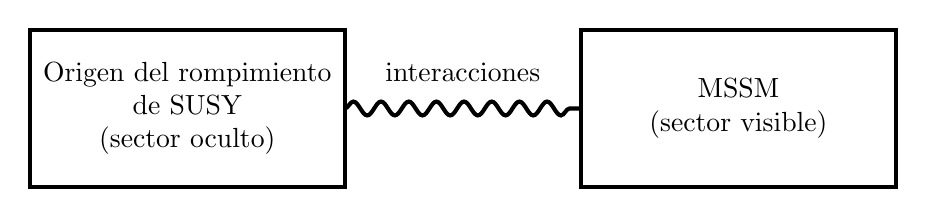
\begin{tikzpicture}

  \draw[line width=1.5] (0,0) rectangle (4,2) node[midway,align=center] (r1) {Origen del rompimiento\\ de SUSY\\ (sector oculto)};
  \draw[line width=1.5] (7,0) rectangle (11,2) node[midway, align=center] (r2) {MSSM\\ (sector visible)} ;

  \draw[line width=1.5,decorate,decoration={snake}] (4,1) -- (7,1) node[midway,above=.2cm] {interacciones};

\end{tikzpicture}

\end{figure}

Existen muchas propuestas de como estas interacciones
mediadores puede ser. Una de estas (e historicamnete la mas popular)
es que estas interacciones son gravitacionales (SUGRA). Mas precisamente
estas asociados con la nueva física, incluyendo a la gravedad, que
aparece cerca de la escala de Planck. En este escenario

Una segunda posibilidad es que estas interacciones mediadores sean
as interacciones de gauge electrodébil y QCD ordinarias. En estos
escenarios donde el rompimiento de supersimetría esta mediado por
campos de gauge (GMSB), los términos soft del MSSM provienen de
diagramas a un loop que involucran algunas partículas mensajeras.

Si tenemos en cuenta a la gravedad, la supersimetría tiene que ser
promovida a una simetría local. Esta teoría supersimétrica local
es llamada \emph{supergravedad}. Esto unifica necesariamente las
simetrías espacio-temporales ordinarias de la Relatividad General
con las transformaciones locales supersimétricas. En esta teoria,
el graviton de spin 2, tiene un supercompa\~nero fermión de spin 3/2
llamado \emph{gravitino}. Mientras la supersimetría no este rota,
el graviton y el gravitino son no masivos con dos estados de helicidad
de spin. Una vez que SUSY es espontáneamente rota, el gravitino adquiere
una masa absorbiendo el goldstino, que se convierte en sus componentes
longitudinales (helicidad $\pm 1/2$). Este mecanismo es llamado \emph{super-Higgs},
y es el análogo al mecanismo de Higgs ordinario de las teorías de gauge,
donde los bosones de gauge $W^\pm$ y $Z^0$ en el {\SM} adquieren
masa absorbiendo los bosones de Nambu-Goldstone asociados con la
invarianza de gauge electrodébil espontáneamente rota. La masa del
gravitino es tradicionalmente llamada $m_{3/2}$, y puede ser estimada
como

\begin{equation}
  m_{3/2} \sim \avg{F} / M_P
\end{equation}

Esto implica distintos valores esperados para la masa del gravitino
dependiendo el modelo de mediadores propuesto. En modelos de mediación
por gravedad, la masa del gravitino es comparable a la masa de las
sparticulas del MSSM, por lo tanto es esperado que sea de al menos
el orden de 100 \gev. Sus interacciones van a ser de intensidad
gravitacional, el gravitino no juega ningún rol en física de
colisiona dores, pero puede ser importante en cosmología.

En contraste, los modelos GMSB predicen un gravitino mucho mas
liviano que las sparticulas del MSSM si $M_\text{mess} \ll M_P$.
En este caso, el gravitino es la LSP, y todas las sparticulas
del MSSM van a decaer eventualmente en un estado final que incluye
el gravitino.








%------
% GMSB
%------
\section{GMSB} %%Modelos de rompimiento de supersimetría mediados por campos de Gauge}

\note{Referencia: arxiv:9801271}

En los modelos de rompimiento de la supersimetría mediado por campos de gauge
(GMSB), las interacciones ordinarias de gauge son los responsables de la
aparición del rompimiento de la supersimetría \emph{soft} en el MSSM.
La idea básica es introducir
nuevos supermultipletes quirales, llamados mensajeros, que se acoplen ...


\subsection{La LSP: El gravitino}

Como resultado del rompimiento espontaneo de la supersimetria, el espectro fisico
contiene un fermion no masivo de spin 1/2, el goldstino. Cuando la teoria supersimetrica
global esta acoplada a la gravedad y promocionada a una teoria supersimetrica local,
el goldstino provee los modos longitudinales de spin 3/2 del graviton: el gravitino.
Como resultado de este mecanismo de super-Higgs, el gravitino adquiere una masa
que bajo la condicion de la anulacion de la constante cosmologica esta dada por:

\begin{equation}
  m_{3/2} = \frac{F_0}{\sqrt{3}M_P}
\end{equation}
%
donde $M_P = (8\pi G_N)^{-1/2} = 2.4 \times 10^{18} \gev$ es la masa reducida de Planck.
Y $F_0$ es la contribucion total del VEV de rompimiento de SUSY de los campos auxiliares
normalizado de tal forma que la energia de vacio de la teoria supersimetrica global es
$V = F_0^2$...

En los modelos GMSB, el gravitino es la particula supersimetrica mas liviana (LSP) para
cualquier valor relevante de $F$. Si la paridad-R es conservada, todas las particulas
supersimetricas van a seguir cadenas de decaimineto que terminan en gravitinos.

%% Para
%% calcular la tasa de decaimiento
%% La caracteristica mas representativa de los modelos GMSB es el gravitino liviano

\subsection{La NLSP}

\hl{La NLSP puede ser cualquier .... Focus on neutralino NLSP}

La segunda particula supersimétrica mas liviana (NLSP) juega un rol
fundamental en la fenomenología de los modelos GMSB. Asumiendo que se
conserva la paridad-R, todas las particulas supersimétricas van a decaer
rapidamente en una cascada hasta la NLSP, y esta va a decaer en un gravitino
via interacciones 1/F. Por este motivo, la naturaleza de la NLSP
determina las signaturas en los colisionadores y algunas propiedades
cosmologicas del GGM. La NLSP puede ser, dependiendo de la eleccion \note{ref a http://arxiv.org/pdf/hep-ph/9801271v2.pdf}
de los parametros, el neutralino, el stau, y en algunas regiones del
espacio de parametros muy restrictivas, el sneutrino.

En el caso de que sea neutralino, esta tiene, en la mayoria de los
casos, una componente dominante de bino, ya que el cociente $\mu/\M{1}$
es generalemente mayor a 1. %Una excepcion ocurre para N grande y M y lambda
%chico?

Las tazas de decaimiento del {\ninoone} NLSP son:\note{pongo las formulas?}

\begin{align}
  \Gamma (\ninoone \to \gamma \gravino) =
\end{align}

Las particulas, que aunque no son NLSP, tienen un decaimiento dominante en
su companero supersimetrico y el {\gravino} se denominan \emph{co-NLSP}.
Para valores grandes de $\tan \beta$, las dos primeras generaciones de
sleptones decaen como $\susy{\ell}_R \to \ell \tau \stau$ y el stau
es la ``unica'' NLSP. Otra posibilidad es que el {\ninoone}, aunque no sea
la NLSP, esta degenerado en masa con el {\stau}, y su decaimiento dominante
sea a un foton y un goldstino. En este caso {\stau} y {\ninoone} son co-NLSP.

La posibilidad de que el sneutrino sea NLP es muy marginal. Requiere valores
de $N$ tan grandes y valores tan chicos de $\Lambda$ que el descubrimiento de
SUSY deberia darse muy pronto. En este caso el sneutrino decae en un neutrino
y un goldstino.

Todos estos casos corresponden a una fenomenologia completamente diferente en
los experimentos de altas energias.

\subsection{Neutralino NLSP}

En el caso de que la NLSP sea el neutralino, la fenomenología se puede entender
mejor yendo a algunos limites simplificados de los autoestados. De esta forma
los distintos tipos son:

\begin{itemize}
\item bino NLSP
\item wino co-NLSP
\item higgsino NLSP
\end{itemize}

%% We will formulate minimal spectra in this paper which allow for significant strong SUSY production at the early LHC,
%% and populate the many final states   available to general neutralino NLSPs.

%% El espacio de parámetros consiste esencialmente en una escala de producción de color (masa del gluino)
%% y la masa de la NLSP. Todas las demás sparticulas se desacoplan que no son esecnailes en la producción
%% de la signatura de interés. De alguna forma, esto es similar a utilizar ``modelos simplificados'' como
%% se utilizan en muchos estudios fenomenológicos y experimentales. \todo{add references?}

El neutralino NLSP decae a $X + \gravino$, donde $X=\gamma, Z, h$, y los
diferentes autoestados de gauge se caracterizan por tener distintos
BR a las diferentes $X$.

  %% The branching fractions of the bino-like and wino-like neutralino NLSP are shown in the figure.
  %% \includegraphics[width=0.5\textwidth]{br_bino}
  %% \includegraphics[width=0.5\textwidth]{br_wino}

Los binos decaen a fotones con un BR $\sim \cos^2\theta_W$, con una componente menor a Z's, con
BR $\sim \sin^2\theta_W$.
Por otro lado estos BR se intercambian en el caso de que la NLSP sea el wino neutro, que decae
mayormente a Z's.
Si la NLSP es higgsino, este decae en forma dominante a Z o $h$, con branching ratio que depende
en el valor de $\tan\beta$ y del signo de $\mu$. Hay tres casos:

\begin{itemize}
\item El decaimiento del higgsino es dominantemente a Z a bajo $\tan\beta$ y $\mu$ positivo,
\item rico en $h$ a bajo $\tan\beta$ y $\mu$ negativo,
\item y una mezcla de $Z$ y $h$ a moderado y alto $\tan\beta$.
\end{itemize}

Cuando la NLSP es mayormente wino, hay una muy pequena degeneracion entre el wino neutro y el
cargado. Cuando esto pasa, el decaimiento de tres cuerpos al wino neutro comienza
a ser excluido, y el wino cargado prefiere decaer directamente a $W^{\pm}$ y un gravitino.
En otras palabras, el wino neutro y el wino cargado se vuelve co-NLSPs, y los estados finales van
a contener $W$'s, $Z$'s y fotones.

Por otro lado, la degenraci\'on entre los higgsinos cargados y neutros es generalmente mayor, de modo
que solo el neutralino mas livinao decae directamente en gravitino.

El espectro simplificado se muestra en la figura. Básicamente consideramos variar
la masa del gluino (\M{3}) y la masa de la NLSP (\M{1}, \M{2} ó $\mu$ dependiendo
si la NLSP es bino, wino ó higgsino, respectivamente). Todos los demás estados
están desacoplados (sus masas seteadas a 2.5 \tev), ya que no juegan un rol importante
en las signaturas que nos interesan.

\begin{figure}[h]
  \centering
  \includegraphics[width=0.5\textwidth]{figures/figura}
\end{figure}

%% We emphasize that these minimal
%% parameter spaces do correspond to physical models, since the entire GGM parameter space
%% was covered by a perturbative messenger model in [10]

%% Our simplified spectra are characterized by several types of SUSY production, with NLO
%% cross-sections shown in figure 4. For each benchmark, there is colored gluino production, with
%% rate set by the gluino mass. For the wino and higgsino NLSPs, there is also the possibility of
%% direct NLSP production with electroweak cross-sections. While the Tevatron currently has
%% the advantage here because of its much larger dataset, we will see below that the LHC will
%% have sensitivity to electroweak production with & 1 − 5 fb −1

\subsection{Bino NLSP}

The dominant decay mode for the bino NLSP is to a photon and gravtitino. The leading channel is the diphoton signature because of the large branching ratio of about $(\cos^2\theta_W)^2 \sim 0.6$,
and low SM background.

\subsection{Wino co-NLS}

\subsection{Z-rich higgsino NLSP}

Higgsinos introduce  an important difference in the topology of the gluino decays. In the bino and wino benchmarks, the gluino decayed 3-body to the neutralino and two jets,
through an off-shell squark. But the higgsino couples predominantly yo heavy flavor, where the mass of the top can squeeze out the 3-body decays. In this regime, the dominant gluino decay is
a one-loop two body decay, $\gluino\to g\susy{H}_{1,2}$.

\subsection{Other higgsino types}

The higgsino dominantly decays to Z's at low tanb and positive mu. For larger values of tanb, the higgsino decays to a roughly even mixture of Z's and h's


\section{Producción de partículas supersimétricas en el LHC}

%% \todo[inline]{add gluino production.decays diagrams, two-body, three-body}

En los colisionadores hadronicos, las sparticulas pueden ser producidas en pares a partir
de colisiones de partones de electroweak strength.

\begin{align}
  &q\bar{q} \, \to \, \chinop \chinom, \nino \nino \\
  &q\bar{q} \, \to \, \susy{\ell}^{+}_{i}\susy{\ell}^{-}_{j}, \susy{\nu}_{\ell}\susy{\nu}^{*}_{\ell}
\end{align}

y reacciones de QCD strength:

\begin{align}
  gg \qquad &\to \qquad \gluino\gluino, \susy{q_i}\susy{q_j}^{*}, \label{eq:gg}\\
  gq \qquad &\to \qquad \gluino\susy{q_i}, \label{eq:gq} \\
  q\bar{q} \qquad &\to \qquad \gluino\gluino, \susy{q_i}\susy{q_j}^{*}, \label{eq:qqbar} \\
  qq \qquad &\to \qquad \susy{q_i}\susy{q_j}, \label{eq:qq} \\
\end{align}

Las dos primeras reacciones obtienen contribuciones de los vectores bosonicos
electrodebiles en el canal $s$, y los de la primera tambien tienen contribuciones
del canal $t$ que son menos importantes en la mayoria de los modelos.
Los procesos en \eqref{eq:gg,eq:gq,eq:qqbar,eq:qq} tienen contribuciones del intercambio
del correspondiente squark o gluino en el canal $t$, y \eqref{eq:gg} y \eqref{eq:qqbar}
tambien tientn contribuciones de gluones en el canal $s$.


En Tevatron, los procesos de produccion de charginos y neutralinos tienden a tener
mayores seccion eficaz, a menos los squarks o el gluino sean muy liviano (menos a 300 \gev,
masas que ya se encuentran excluidas por el LHC). En el LHC, la situacion es opuesta, con la
produccion de gluinos y squarks dominante por medio de gluon-gluon y gluon-quark fusion.
En ambos colisionadores, puede haber produccion asociada de chargino o neutralino junto con
un squark y un gluino, pero la mayoria de los modelos predicen que la seccion eficaz




%% \section{arxiv 0911.4130}
%% SUSY breaking in the MSSM introduces ~ 100 parameters

%% Una de las caracteristicas mas caracteristica de gauge medaition es el gravitiino liviano $m_{3/2}<<M_\text{weak}$.
%% Esto asegura que los efectos de gauge mediation dominan por sobre  las contribuciones suprimidas de
%% Plank de la mediacion por gravedad. Esto implica que la la supercompanera mas liviana del MSSM es realemnte
%% la NLSP, que siempre tiene que decaer en un gravitino mas su compnera del {\SM}. El gravitino siempre
%% va a escapar del detector, dejando una gran cantidad de energia faltante. Mientras tanto , la companera
%% del {\SM} va a ser por lo general central y enrgetico (asumiendo que la NLSP decae promptly), ya
%% que es en general mucho mas liviano que la NLSP. Y dado que en cada evento se producen un par de NLSP,
%% las inclusive signautes en los colisionadores de GMSB van a ser largamente determinadas por la naturaleza
%% de la NLSP.

%% En 20\todo{Check ref 20} se estudia la cuestion de como formular gauge mediation en una forma que sea model-independent.
%% Esto resulto en el desarrollo de General Gauge Mediation (GGM), en el cual el espacio entero de los
%% posibles modelos de guage medation  pueden ser investigados sin tener que basarse en modelos especificos.

%% El conjunto completo de paramentros independientes de gauge mediation puede derivarse: tres masas
%% de gauginos complejas $M_{1,2,3}$ y tres parametros reales que controlan las masas cuadradas de
%% los 5 sfermiones $m^2_{Q,U,D,L,E}$. Tambien se ha argumentado que en el marco de GGM, los terminos
%% trilineares $A$ son siempre pequenos.

%% Cualquier spartícula del MSSM puede ser la NLSP en {\GM}. Si la NLSP es una sparticula con carga
%% de color, la signatura inclusiva (asumiendo decaimientos prompt) es dijet + \met.

%% La NLSP también puede ser un slepton, aunque es muy chica la produccion directa de sleptones en
%% el LHC, pero si pueden producirse en cascadas de decaimiento originadas en producción de pares de
%% sparticulas con color, o charginos y neutralinos. Por lo tanto las busquedas de sleptones tienen
%% que ser necesariamente mas dependientes del modelo, involucrando mas parametros del espectro.

%% Y finalmente, tenemos la posibilidad de que la NLSP sea un neutralino o chargino. Los charginos
%% s\'olo pueden ser NLSP en regiones muy peque\~nas del espacio de par\'ametros. Entonces nos queda
%% como la ultima posibilidad que la NLSP sea del tipo neutralino.

%% En general, el neutralino puede ser una mezcla arbitraria de los autoestados de gauge bino, wino
%% y higgsino. Entonces el hecho de tener un par de nuetralinos en cada evento de SUSY, da lugar a
%% signatras inclusivas involucrando combinaciones (adecuadamente elegidas) de $\gamma + \met$,
%% $Z + \met$ o $h + \met$. Una de las signaturas mas estudiadas tanto en Tevatron como el LHC ha sido
%% $\gam\gam + \met$. Adicionalmente, si la degeneracion entre las masas del neutralino NLSP y el chargino
%% mas liviano, puede haber cadenas de decaimiento que terminen con un estado final de $W^{\pm} + \met$.


%%\section{De la Nota+Paper}
%% Las teorias Gauge Mediated Symmetry Breaking (GMSB) \cite{Dine:1981gu,AlvarezGaume:1981wy,%
%%   Nappi:1982hm,Dine:1993yw, Dine:1994vc,Dine:1995ag}
%% consideran un sector oculto en el cual la supersimetria esta rota y la rotura de la simetria
%% es comunicada a los sectores visibles a traves de las interacciones de bosones de gauge del
%% modelo estandard.


%% Theories of Gauge Mediated Symmetry Breaking (GMSB)  presume a hidden sector in which supersymmetry is
%% broken and the symmetry breaking is communicated to the visible sectors through Standard Model gauge boson
%% interactions. Such theories are especially attractive because the hypothesis of an intermediate hidden sector
%% suppresses the magnitude of flavor-changing neutral currents. The lightest supersymmetric particle (LSP) in GMSB
%% is the ultra-light gravitino (\gravino), which under certain circumstances is a viable dark matter candidate \cite{Goldberg:1983nd,Ellis:1983ew}.
%% The \gravino\ has a derivative coupling to each particle and its superpartner with an interaction strength inversely
%% proportional to $\sqrt{F}$, where $F$  is a vacuum expectation value of an auxiliary field which determines the
%% magnitude of supersymmetry breaking in the vacuum state.



%% %% If the \ninoone\ is bino-like, the main decay mode is $\ninoone\to\gam\gravino$. If the \ninoone\ is
%% %% higgsino-like, it decays as $\ninoone\to h\gravino$. In addition, since the longitudinal polarisation component of the Z boson is also a Goldstone
%% %% mode of the Higgs field, a higgsino-like neutralino can also decay as $\ninoone\to Z\gravino$.
%% Consecuentemente un par de {\ninoone} producidos en un colisionador pueden dar lugar a estados finales
%% de dos bosones ($hh$, $h\gam$, $hZ$, $Z\gam$, $ZZ$, $\gam\gam$) + \etmiss.



%% %% %The next-to-lightest supersymmetric particle (NLSP)
%% %% %%defines the phenomenology of these models, and
%% %% % is almost always the lightest neutralino \ninoone, often assumed to be a bino-like particle. The bino is the supersymmetric
%% %% % partner of the U(1) gauge �eld, coupling to the photon and Z boson with strengths that are determined by the Weinberg
%% %% % mixing angle. This results in the \ninoone decaying predominantly to the LSP and a photon. Assuming that R-parity \cite{} is
%% %% % conserved, the classical signature of GMSB is, therefore, events with two energetic isolated photons and large missing
%% %% % transverse momentum (\etmiss). Searches for such a signature at the LHC and the Tevatron established strong
%% %% % experimental constraints on GMSB models \cite{}.

%% %% The present analysis is motivated by the bino-higgsino admixture neutralino decay signatures predicted by General Gauge Mediation (GGM) models,
%% %% namely a final-state signature that consists of a photon, jets, and high \MET. The event selection described in \Sec \ref{sec:event_selection},
%% %% has been designed to maximize the sensitivity to a small signal with this general topology. Any imposition of model-tailored selection cuts has been
%% %% avoided, trying to keep the analysis as model independent as possible. However, an interpretation in the framework of a specific model is unavoidable.
%% %% A grid of GGM signal points is simulated with a specific set of benchmark parameter values that covers the region in which signal can be established.
%% %% The sensitivity of the analysis is evaluated using this grid of points.

%% %% In this particular region of the GGM model space, the lightest neutralino is a mixture of bino and higgsino. The neutral wino is much heavier so it
%% %% does not contribute. Due to the Weinberg mixing angle in the Standard Model, the bino component of the lightest neutralino couples to both the photon and the Z.
%% %% The gluino is regarded as the only relevant coloured sparticle in order to set a conservative limit on the gluino mass. All squark soft masses are set to 2.5 TeV.
%% %% The other model parameters are set to M$_2$=2.5 \tev, $\tan\beta$=1.5 and $c\tau_{\mathrm{NLSP}} < 0.1$ mm. The latter assures the neutralino is decaying promptly
%% %% and is achieved by making the gravitino sufficiently light ($m_{\tilde{G}}=10^{-9}$ \gev). All trilinear coupling terms are set to zero and masses of sleptons
%% %% are set to 2.5 \tev. The Higgs boson is in the decoupling regime with $m_{A}$ = 2 \tev~ and $m_{h}$ = 126 \gev. The last follows the recently measured value
%% %% for the SM Higgs boson at the LHC \cite{ATLAS-CONF-2013-014,CMS-PAS-HIG-14-009}. In gauge mediated SUSY scenarios several mechanisms exist \cite{Craig:2011yk,Auzzi:2011eu,Csaki:2012fh,Larsen:2012rq,Craig:2012hc}
%% %% to generate a Higgs boson mass as high as this observed value, without changing the phenomenology of the models here considered. No significant effect on the mass spectrum
%% %% has been indeed observed when varying this value within a $\pm 10~$ \gev\ range.

%% %% \Mone\ and $\mu$ determine the lightest neutralino mass, and are related in such a way that the branching ratios of the \ninoone\ are approximately constant,
%% %% resulting in ${\rm BR}(\ninoone \to \gam + \gravino) \approx 50\%$, ${\rm BR}(\ninoone \to Z + \gravino) \approx 49\%$ and ${\rm BR}(\ninoone \to h + \gravino) \approx 1\%$,
%% %% numbers which vary by $\pm 1\%$ throughout most of the grid (\Fig \ref{fig:br_n1_x_grav}). For light neutralinos ($<200\gev$) the Higgs production is highly
%% %% suppressed and ${\rm BR}(\ninoone \to \gam + \gravino)$ starts falling up to 40\%. The value of $\mu$ must also be positive in order to disfavor the branching ratio
%% %% to the Higgs boson, which would lead to a signature already covered by a dedicated analysis in ATLAS \cite{Aad:2012jva}. Similarly, the branching ratio for
%% %% ($\ninoone \to \gam + \gravino$) is such that maximizes the single photon final state. At larger values the diphoton topology starts to be favoured, which has been
%% %% extensively searched for in the past \cite{Aad2012519,Aad:2011kz}. This leaves $M_3$ and $\mu$ as the only two free parameters of the model, spanning the space
%% %% within $150\gev < m_{\ninoone} < 1250 \gev$ and $800\gev < m_{\gluino} < 1300 \gev$, with $m_{\ninoone} < m_{\gluino}$. The granularity of the simulation in each
%% %% dimension is shown in \Tab\ \ref{tab:signal_pars}, with the resulting value for the gluino and neutralino masses.

%% %% The full mass spectrum, the gluino and neutralino branching ratios and decay widths are calculated from
%% %% these set of parameters using SUSPECT v2.41 \cite{Djouadi2007426}, SDECAY v1.3b \cite{Muhlleitner:2004mka}
%% %% and HDECAY v3.4 \cite{Djouadi:1997yw}, run as part of the SUSYHIT package v1.3 \cite{Djouadi:2006bz}.
%% %% An example of the mass spectrum in the configuration is shown in \Fig \ref{fig:mass_spectra}, for one of
%% %% the signal grid points. The total decay branching ratios for \gluino-initiated \ninoone\ production are
%% %% shown in \Fig \ref{fig:br_gl_n1}, for 2-body\footnote{only effectively, the gluino decays through a virtual
%% %% quark-squark loop in this case.} and 3-body gluino decays.
%% %% Simulated events were generated with HERWIG++ v2.5.2 \cite{Bahr:2008pv} for the 124 signal points in the
%% %% grid (5K per each), using the CTEQ6L1 \cite{Nadolsky:2008zw} parton density distributions. A generator level
%% %% filter requiring a photon with $p_{T}>100~$ \gev\ was applied to get higher statistics, specially at low neutralino
%% %% mass. The filter efficiency for all simulated points are shown in \Tab \ref{tab:signal_filter_eff}.

%% %% Signal production cross sections and uncertainties were calculated using the SUSYSignalUncertainties package \cite{SUSYsigunc}. Cross sections
%% %% for the signal processes involving the production of gluino pairs are calculated to next-to-leading order (NLO)
%% %% in the strong coupling constant, adding the resummation of soft gluon emission at next-to-leading-logarithmic
%% %% accuracy (NLO+NLL) \cite{Beenakker:1996ch,Kulesza:2008jb,Kulesza:2009kq,Beenakker:2009ha,Beenakker:2011fu}.
%% %% The EWK $\tilde{\chi}\tilde{\chi}$ production cross sections are calculated to next-to-leading order in the strong coupling constant (NLO) using PROSPINO v2.1~\cite{Beenakker:1999xh}.
%% %% %are computed at NLO with Prospino v2.1 \cite{Beenakker:1996ed}.
%% %% The cross sections and uncertainties are tabulated in \Tab \ref{tab:signal_xs_strong} and \ref{tab:signal_xs_ewk}, and shown in \Fig \ref{fig:signal_xs_strong} and \ref{fig:signal_xs_ewk}, for the strong and EWK production respectively.
%% %% The total nominal cross section and the relative contribution of EWK produced processes are also shown in \Fig \ref{fig:signal_xs_total}.
%% %% The total uncertainty is taken from an envelope of cross section predictions using different PDF sets and factorisation and renormalisation scales, as described in \Ref \cite{Kramer:2012bx}. More details of the uncertainties treatment are given in \Sec \ref{sec:syst_signal}. %The dependence of the cross section with $M_3$ is also shown in Fig. \ref{fig:signal_xs}.

%% %% All signal samples have been simulated with the faster, parametrized detector simulation ATLFAST-II \cite{Richter-Was:683751}. Derived datasets in the {\sc NTUP\_SUSY}
%% %% format are used throughout this analysis, with the configuration tag p1328.









%% %% For GGM, the NLSP can be formed from an admixture of any of the SUSY partners
%% %% of the gauge boson and Higgs states.
%% %% In this study, three cases are assumed for the
%% %% composition of the NLSP. For the first case, the NLSP is assumed to be
%% %% purely bino-like (the SUSY partner of the SM U(1) gauge boson). For the
%% %% second case, the NLSP is assumed to be an admixture
%% %% of the bino and a higgsino that is assumed to be the SUSY partner
%% %% of the SM Higgs boson $h$. For the final
%% %% case, the NLSP is assumed to be a degenerate triplet
%% %% of wino states (the SUSY partners of the SM SU(2) gauge bosons).
%% %% In this paper, the neutral NLSP is denoted $\neutralino$ irrespective
%% %% of its composition. For the case that
%% %% the NLSP is a degenerate triplet, the charged NLSP states are denoted $\chargino$.

%% %% For the case that the NLSP is a bino,
%% %% the final decay in each of the two cascades in a GGM event would predominantly be
%% %% $\neutralino\to\gamma+\gravitino$, leading
%% %% to final states with $\gamma\gamma+\met$.
%% %% For the case that the NLSP is a mixture of the bino
%% %% and higgsino, both the possibilities that the higgsino mass
%% %% parameter $\mu$ is less than or greater than zero are explored.
%% %% In the former case, the final decay in the cascade would include
%% %% a significant contribution from $\neutralino\to h + \gravitino$
%% %% with the subsequent decay $h \to \bbbar$, leading to final
%% %% states with a photon, multiple $b$-jets, and $\met$.
%% %% %(here `$h$' is assumed to have the couplings and branching fractions
%% %% %equal to those expected for the SM Higgs boson).
%% %% The latter case can produce scenarios for which the
%% %% final decay in the cascade can be relatively evenly split
%% %% between $\neutralino\to\gamma+\gravitino$ and
%% %% $\neutralino\to Z + \gravitino$, leading to final states with
%% %% a photon, multiple jets (including two from the hadronic decay of the $Z$ boson)
%% %% that typically do not arise from $b$ quarks,
%% %% and $\met$.
%% %% For the case that the NLSP is a degenerate set of three wino states,
%% %% the final step in the cascade includes both charged and neutral wino decays.
%% %% Charged wino decays tend to produce isolated
%% %% leptons, while neutral wino decays produce photons with a wino-to-photon
%% %% branching fraction that is no less than $\sin^2 \theta_W$ for any value of
%% %% the wino mass. Overall, these two wino-NLSP contributions lead to a significant
%% %% number of events with an isolated photon accompanied by an isolated lepton.
%% %% Of the five %seven
%% %% GGM models considered here, two (the `gluino-bino' and `wino-bino' models) %three
%% %% incorporate a purely bino-like NLSP, two (the `higgsino-bino' models)    %three
%% %% incorporate an NLSP that is a higgsino-bino admixture, and one (the `wino-NLSP' model)
%% %% incorporates a wino-like set of NLSPs; in all cases
%% %% the mass of the NLSP state is considered to be a free parameter
%% %% of the model.
%% %% A summary of these models,
%% %% including their motivating experimental signatures, is presented in Table~\ref{tab:GGM_models}.

%% %% The two %three
%% %% GGM models incorporating a bino-like NLSP
%% %% are the focus of the diphoton analysis. For these models,
%% %% one other set of SUSY partner states is taken to be potentially
%% %% accessible in 8 TeV {\it pp} collisions, while
%% %% all other SUSY mass parameters are decoupled (set to
%% %% inaccessibly large values). For both %all three
%% %% of these bino-like NLSP cases, production
%% %% proceeds solely through this set of SUSY partners,
%% %% with the NLSP appearing in the subsequent
%% %% decays of the produced SUSY partner states. For the gluino-bino
%% %% model, the set of partners is composed of a degenerate octet of
%% %% gluinos (gluon partners).
%% %% %Also considered is a `squark-bino' model for which production proceeds through a mass-degenerate
%% %% %set of squarks (quark partners),
%% %% %including all
%% %% %squark flavors and chiralities of squarks excepting
%% %% %the right-handed up-type squark,
%% %% %whose mass is decoupled.
%% %% For the `wino-bino' model, the set of partners is composed
%% %% of a degenerate triplet of wino states
%% %% \neutralinotwo, \chargino, and is dominated by the production
%% %% of \chiplus\chiminus and \neutralinotwo\chargino.
%% %% For both %all three
%% %% of these models, the masses of these produced states
%% %% are considered to be free parameters along with that of the chosen
%% %% \neutralino state, the latter of which is constrained to be less
%% %% than those of the produced states.
%% %% This results in a SUSY production
%% %% process that proceeds through the creation of pairs of the higher-mass
%% %% states, which subsequently decay through
%% %% short cascades to the NLSP \neutralino states. Other SM
%% %% objects (jets, leptons, photons) may be produced in these cascades.
%% %% The \neutralino branching fraction
%% %% to $\gamma$ + \gravitino is 100\% for $m_{\neutralino} \to 0$ and
%% %% approaches $\cos^2 \theta_W$ for $m_{\neutralino} \gg m_Z$, with
%% %% the remainder of the \neutralino sample decaying to $Z$ + \gravitino.
%% %% For all \neutralino masses, then, the branching fraction is dominated
%% %% by the photonic decay, leading to the diphoton-plus-\met signature.
%% %% For these models with a bino-like NLSP, typical production and decay channels for strong (gluino) and
%% %% electroweak (wino) production are exhibited in Fig.~\ref{fig:feynman_bino}.

%% %% \begin{figure}[tp]
%% %%   \begin{center}
%% %%     \includegraphics[width=0.45\textwidth]{gogo-qqqqphphGG-GMSB} ~~
%% %%     \includegraphics[width=0.45\textwidth]{C1C1-WWphphGG-GGM}
%% %%   \end{center}
%% %%   \caption{
%% %% Typical production and decay-chain processes for the gluino-production (left)
%% %%       and electroweak-production (right) instances of the
%% %%       GGM model for which the NLSP is a bino-like neutralino.
%% %% %      For the higgsino-bino models, the final
%% %% %      step of the cascade (the \neutralino decay) would have a
%% %% %      probability of order 50\% for producing a Higgs
%% %% %      (for the model with $\mu < 0$) or $Z$ (for the model with $\mu > 0$)
%% %% %      boson.
%% %%     \label{fig:feynman_bino}
%% %%   }
%% %% \end{figure}

%% %% \begin{figure}[tp]
%% %%   \begin{center}
%% %%     \includegraphics[width=0.45\textwidth]{gogo-qqqqbbphGG-h} ~~
%% %%     \includegraphics[width=0.45\textwidth]{gogo-qqqqphZGG-GMSB}
%% %%   \end{center}
%% %%   \caption{
%% %%     Typical production and decay-chain processes for the gluino-production
%% %%     and electroweak-production instances of the
%% %%     GGM model for which the NLSP is a higgsino-bino neutralino admixture.
%% %%     For the model with $\mu < 0$ (left), the final
%% %%     step of the cascade (the \neutralino decay) would have a
%% %%     probability of order 50\% of producing a Higgs boson rather than a
%% %%     photon or $Z$ boson; for the model
%% %%     with $\mu > 0$ (right), the \neutralino decay would have a
%% %%     probability of order 50\% of producing a Z boson rather than a photon.
%% %%     \label{fig:feynman_higgsino_bino}
%% %%   }
%% %% \end{figure}

%% %% \begin{figure}[tp]
%% %%   \begin{center}
%% %%     \includegraphics[width=0.45\textwidth]{C1N1-phlvGG-W}
%% %%   \end{center}
%% %%   \caption{
%% %% Typical production and decay-chain processes for the wino-NLSP model.
%% %% In this model, the \neutralino is a pure \winon state, while the
%% %% \chargino are the two charged wino states.
%% %%     \label{fig:feynman_wino}
%% %%   }
%% %% \end{figure}

%% %% %Three
%% %% The higgsino-bino GGM models incorporate an NLSP composed of
%% %% a higgsino-bino admixture, as well as
%% %% %including `gluino-higgsino'%, `squark-higgsino'
%% %% %and `gluino-higgsino-jets' models that incorporate degenerate sets
%% %% a degenerate octet of gluinos %and squarks
%% %% identical in nature to those of the
%% %% gluino-bino model. % and squark-bino models, respectively.
%% %% For the first %two
%% %% of these models, which is the focus of the photon+b analysis,
%% %% the higgsino mass parameter $\mu$ is required to be negative, and the composition
%% %% of the NLSP is set by adjusting $\mu$ and the GGM U(1) mass parameter
%% %% $M_1$ so that a constant ratio of the branching fraction of $\neutralino \to h + \gravitino$
%% %% to that of $\neutralino \to \gamma + \gravitino$ is maintained at
%% %% approximately 1.7:1 over the full range of NLSP masses.
%% %% In the limit that $m_{\neutralino} \gg m_Z$, the NLSP
%% %% branching fractions to $h + \gravitino$, $\gamma + \gravitino$,
%% %% and $Z + \gravitino$ approach 56\%, 33\%, and 11\%, respectively.
%% %% The GGM SU(3) mass parameter $M_3$ bears a direct relation to the
%% %% gluino mass, and is taken to be a free parameter in this $\mu < 0$ higgsino-bino
%% %% model, with all squark states decoupled.
%% %% %For the squark-higgsino model, the gluino
%% %% %mass and the mass of the right-handed up-type squark are decoupled, with the
%% %% %remaining squark masses treated as a single free parameter. For both of these models,
%% %% The GGM SU(2) mass parameter $M_2$ is set to a value of 2.5 TeV.
%% %% Four other electroweak gaugino states typically lie
%% %% within 25 GeV of the \neutralino NLSP: the two lightest charginos \chargino, and two
%% %% additional neutralinos \neutralinotwo and \neutralinothree.
%% %% The pair production of gluinos or any of these four additional gaugino
%% %% states leads to decays to the \neutralino via
%% %% cascades involving SM particles.

%% %% For the second of the higgsino-bino models, which is
%% %% the focus of the photon+j analysis, the $\mu$ parameter is
%% %% chosen to be positive, which suppresses the $h + \gravitino$
%% %% decay mode of the higgsino. As for the models described above,
%% %% the NLSP mass is taken to be a free parameter.
%% %% The $M_1$ and $\mu$ parameters are adjusted so that the branching
%% %% fractions of the $\neutralino$ to $\gamma + \gravitino$, $Z + \gravitino$
%% %% and $h + \gravitino$ are maintained close to 50\%, 49\% and 1\% for
%% %% most values of the $\neutralino$ and gluino masses.
%% %% In this model, the production of gluino pairs can be followed
%% %% by decays to both a single photon and a hadronically-decaying $Z$ boson, producing
%% %% events with a single isolated high-energy photon accompanied
%% %% by two jets.
%% %% In the case that the gluino mass is substantially
%% %% larger than the $\neutralino$ mass, additional jets can
%% %% be produced in the cascade.
%% %% Three additional electroweak gaugino states
%% %% lie close in mass to the \neutralino, allowing for the
%% %% possibility of SUSY production through pairs of these
%% %% states. Such events tend to produce fewer jets than those that proceed through gluino production,
%% %% but in certain regions of the model space can provide a significant
%% %% contribution to data samples selected to isolate the photon-plus-jets
%% %% signature. As for the $\mu < 0$ higgsino-bino model, the value of $M_3$, which is directly
%% %% related to the gluino mass, is taken to be a free parameter, $M_2$ is
%% %% set to a value of 2.5 TeV, and all squark states are decoupled.
%% %% Typical production and decay-chain processes for the two models
%% %% for which the NLSP is a higgsino-bino admixture are shown in Fig.~\ref{fig:feynman_higgsino_bino}.


%% %% Finally, the wino-NLSP model, which is the focus of the photon+$\ell$ analysis,
%% %% incorporates a set of three degenerate wino-like
%% %% NLSPs. This set includes the neutral \winon, which as the lightest
%% %% neutral gaugino is also referred to as the \neutralino,
%% %% as well as the two charged wino states, which form the \chargino states.
%% %% Production proceeds
%% %% %either through pairs of colored sparticles or
%% %% through the direct production of pairs of NLSP states;
%% %% %In either case
%% %% %the decay procedes through two wino-like NLSPs, and as a result
%% %% such events usually contain at least one \winon NLSP. Although
%% %% the \winon couples preferentially to the $Z$ boson relative to
%% %% the photon, the \winon decays into a photon+gravitino final state with unit branching fraction
%% %% for wino mass below that of the $Z$ boson.
%% %% The \winon branching fraction to photon+gravitino approaches
%% %% $\sin^2 \theta_W$ for wino masses far above that of the $Z$ boson.
%% %% Leptons can be produced either through the decays of charged wino
%% %% states, or through the decays of $Z$ bosons that arise from \winon
%% %% decay, leading to a significant probability that the overall final state
%% %% will contain both a photon and a lepton. In this model,
%% %% %a common squark and guino mass is taken as a free parameter
%% %% %along with the wino NLSP mass scale;
%% %% a common wino mass scale is taken as a free parameter, with
%% %% all other GGM mass parameters set to a value of \unit[2.5]{TeV}, except the squark masses,
%% %% which are set to infinity.
%% %% A production and decay diagram typical for this model is shown in Fig.~\ref{fig:feynman_wino}.
%% %% %In all cases, the decay chain
%% %% %procedes through the wino-like NLSP states.


%% %% For all five models considered here, the mass of the gravitino is chosen so that
%% %% the NLSP decay length is never greater than 1 mm. This ensures that all
%% %% particles arising from the decay of the NLSP are prompt, and in particular that
%% %% that the relationship between the point and direction of impact
%% %% of photons from NLSP decay upon the face of the detector is
%% %% consistent with that of a prompt photon (a separate analysis~\cite{Aad:2014gfa}
%% %% searches for GGM models with a longer-lived bino-like NLSP, leading to signatures with non-prompt photons).
%% %% In addition, the ratio
%% %% $\tan \beta$ of the two SUSY Higgs-doublet vacuum-expectation values is set to a value of 1.5;
%% %% %for all but the higgsino-bino model with positive $\mu$ and the wino-NLSP model; for those models
%% %% %$\tan \beta$ is set to 1.5.
%% %% for all five models, the phenomenology relevant to this search is only
%% %% weakly dependent on the value of $\tan \beta$.

%% The scenarios considered in this analysis are the
%% %% ones with only one \gam\ %i.e. $\g Z$ and $\g h$,
%% %% plus two \gravino\ in the final state, in the case \ninoone\ is a bino-higgsino admixture (\Fig \ref{fig:GGM_diagrams} (left)). Further details on the signal models and benchmark points
%% %% considered in this study are given in \Sec \ref{sec:sig_samples}.

%% En a\~no recientes, el esfuerzo por formular GMSB de un modo model-independent has led
%% el desarrollo de general gauge mediation (GGM) \cite{Meade:2008wd,Buican:2008ws}.
%% GGM inlcuye un sector observable con todos los campos de MSSM, junto con un sector oculto
%% que contiene la fuente del rompimiento de SUSY. En GGM, no tiene porque haber una jerarquia
%% entre los estados de color y los de no color, y por lo tanto no hay ninguna restriccion teorica
%% en la masa de los estados de color, aumentando la posibilidad de descubir GGM con los primeros
%% datos del LHC.

Se han realizado muchas búsquedas de estas signaturas en Tevatron
\cite{Abazov:2007ag,Buescher:2005he} y el LHC \cite{Aad:2012zza,
  Aad:2012jva,Aad:2011kz,Aad2012519,leptonphoton7,Chatrchyan:2011wc,
  Chatrchyan:2011ah,tagkey2015503}.

Este trabajo describe la búsqueda de eventos con un fotón aislado muy
energético, jets y energía faltante con todos los datos de las colisiones
$pp$ a una energía de centro de masa de 8 TeV tomadas durante el a\~no
2012 con el detector ATLAS en el LHC, correspondiente a una luminosidad
total integrada de 20.3 \ifb.

Esta búsqueda es complementaria a otras búsquedas en ATLAS con estados finales con
\gam\gam+\etmiss \cite{Aad2012519,ATLAS-CONF-2014-001}, $\gam+e/\mu+\etmiss$ \cite{ATLAS-CONF-2012-144},
$\gam+b+\etmiss$ \cite{Aad:2012jva}, y $Z+\etmiss$ \cite{ATLAS-CONF-2012-152}. El otro gran experimento del
LHC, CMS, también ha realizado estudios similares \cite{CMS-PAS-SUS-12-018,CMS-PAS-SUS-14-004}, aunque solo
en el caso de estados de puro bino o puro wino. %%\todo{Check/update this}

\begin{figure}[h!]
  \centering
  \includegraphics[width=0.31\textwidth]{figures/GGM_diagram_yy}
  \includegraphics[width=0.31\textwidth]{figures/GGM_diagram_yh}
  \includegraphics[width=0.31\textwidth]{figures/GGM_diagram_yZ}
  \caption{Diagramas de producción general de estados finales con
    fotones en SUSY GGM.}
  \label{fig:GGM_diagrams}
\end{figure}
